\chapter{Visibility and contact representations of planar graphs}

\section{$s-t$ numbering}

\begin{defn}
	An $s - t$ numbering (also called a bipolar orientation) of a graph is an acyclic orientation of its edges which has exactly one source (a vertex with no in-coming arcs) and exactly one sink (a vertex with no out-going arcs).
\end{defn}

\begin{prop}
	Every vertex 2-connected graph has an $s - t$ numbering.
\end{prop}

\begin{proof}
	By induction on adding ears, using the Ear Decomposition Lemma. Given the starting cycle, choose two distinct vertices on it (to be the source and the sink) and orient the cycle as two directed paths from the source to the sink. The loop invariant will be that every vertex lies on a directed path from the source to the sink. When adding an ear, orient it in the direction from the source to the sink if both end-vertices of the ear lie on the same path from the source to the sink. If the end-vertices of the ear lie on different paths from the source to the sink, the ear may be oriented either way (but all of its edges in the same direction).
\end{proof}

\begin{thm}
	Every vertex 2-connected plane graph has an $s - t$ numbering and a noncrossing planar drawing such that
	
	\begin{enumerate}[i]
		\item every edge is drawn as a $y$-monotone curve (i.e., every horizontal line crosses the drawing of the edge in at most one point), and
		\item the drawing of every edge is oriented upward in the $s - t$ numbering.
	\end{enumerate}
	\label{thm-1}
\end{thm}

This $s - t$ numbering and a corresponding planar drawing can be constructed in polynomial time.

\begin{comm}
	By saying a plane graph it is meant a planar graph with a given noncrossing drawing in the plane, and it is understood that only drawings which are homeomorphic to the given one are considered, including the choice of the outerface.
\end{comm}

\begin{proof}
	By Ear Decomposition Lemma, the given graph $G$ can be constructed from the cycle bounding its outerface by adding ears. Choose two distinct vertices, say $a$ and $b$, on this cycle, place them in the plane so that they have different $y$-coordinates, the coordinate of a being smaller than the coordinate of $b$, orient the two $a - b$ paths forming the cycle from $a$ to $b$ and draw them as $y$-monotone paths from (the drawing of) a to (the drawing of) $b$.
	
	Then continue adding the ears, orienting their edges and adding them to the drawing constructed while keeping the following loop invariant -- the drawing is homeomorphic to the so far constructed part of $G$, it satisfies i) and ii), all vertices have distinct $y$-coordinates, and each face is bounded by two upward oriented paths connecting its vertices with the lowest and the highest $y$-coordinates (we will refer to these paths as the \textit{left} one and the \textit{right} one). Note that i) and ii) together imply that the drawing of any directed path is $y$-monotone.
	
	When an ear is added, it is added inside a face of the so far constructed part of $G$. Direct the edges of the ear in the direction from the vertex with the lower $y$-coordinate to the vertex with the higher one (the end-vertices of the ear belong to the so far constructed part of $G$ and so they have already been drawn). If the end-vertices belong to the same bounding path (the left one or the right one) of the face they should be draw in, draw the ear as a $y$-monotone curve contouring the bounding path. If the end-vertices belong to different bounding paths, draw the ear as a $y$-monotone curve that contours the path which contains the lower endpoint and traverse the face to the other endpoint almost horizontally close to the $y$-coordinate of this other endpoint, in order to avoid crossings with other edges. It is easy to check that the loop invariant of the construction is fulfilled.
\end{proof}

\begin{figure}[!ht]\centering
	\begin{subfigure}{0.45\textwidth}\centering
		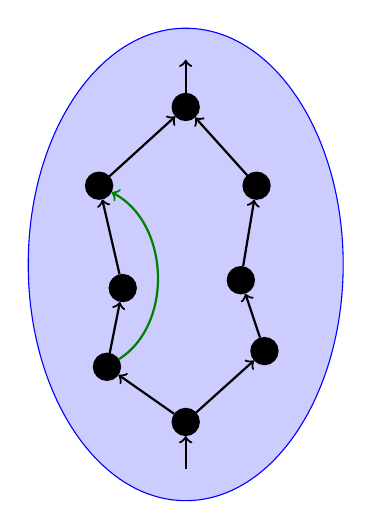
\begin{tikzpicture}[main/.style = {draw, circle, thick, fill}]
			% Draw ellipsoid
			\draw[blue, fill=blue!20] (0,0) ellipse (2 and 3);
			\node[main] (1) at (0,-2) {};
			\node[main] (2) at (-1,-1.3) {};
			\node[main] (3) at (1,-1.1) {};
			\node[main] (4) at (-0.8,-0.3) {};
			\node[main] (5) at (0.7,-0.2) {};
			\node[main] (6) at (-1.1,1) {};
			\node[main] (7) at (0.9,1) {};
			\node[main] (8) at (0,2) {};
			
			\draw[->, thick] (1) edge (2);
			\draw[->, thick] (1) edge (3);
			\draw[->, thick] (2) edge (4);
			\draw[->, thick] (3) edge (5);
			\draw[->, thick] (4) edge (6);
			\draw[->, thick] (5) edge (7);
			\draw[->, thick] (6) edge (8);
			\draw[->, thick] (7) edge (8);
			
			\draw[->, thick] (0, -2.6) -- (1);
			\draw[->, thick] (8) -- (0, 2.6);
			
			\draw[->, thick, color=Green, bend right = 60] (2) edge (6);
		\end{tikzpicture}
	\end{subfigure}
	\begin{subfigure}{0.45\textwidth}\centering
		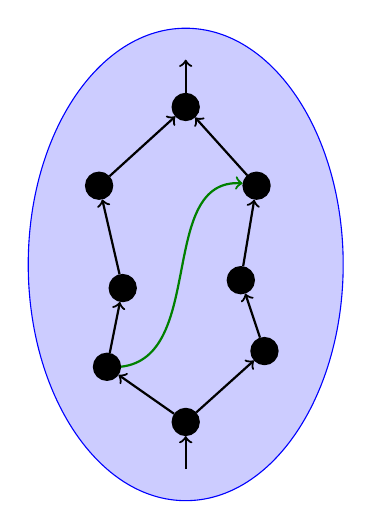
\begin{tikzpicture}[main/.style = {draw, circle, thick, fill}]
			% Draw ellipsoid
			\draw[blue, fill=blue!20] (0,0) ellipse (2 and 3);
			\node[main] (1) at (0,-2) {};
			\node[main] (2) at (-1,-1.3) {};
			\node[main] (3) at (1,-1.1) {};
			\node[main] (4) at (-0.8,-0.3) {};
			\node[main] (5) at (0.7,-0.2) {};
			\node[main] (6) at (-1.1,1) {};
			\node[main] (7) at (0.9,1) {};
			\node[main] (8) at (0,2) {};
			
			\draw[->, thick] (1) edge (2);
			\draw[->, thick] (1) edge (3);
			\draw[->, thick] (2) edge (4);
			\draw[->, thick] (3) edge (5);
			\draw[->, thick] (4) edge (6);
			\draw[->, thick] (5) edge (7);
			\draw[->, thick] (6) edge (8);
			\draw[->, thick] (7) edge (8);
			
			\draw[->, thick] (0, -2.6) -- (1);
			\draw[->, thick] (8) -- (0, 2.6);
			
			\draw[->, thick, color=Green, bend right, out=-50, in=120] (2) edge (7);
		\end{tikzpicture}
	\end{subfigure}
	\caption{An illustration to adding an ear in the construction of an $s-t$ numbering and a corresponding upward drawing.}
\end{figure}

\section{Rectangle visibility representations of planar \\ graphs}

\begin{defn}
	A \textbf{rectangle visibility representation} of a plane graph $G$ is an arrangement of disjoint axes-aligned rectangles in the plane such that the (unions of) horizontal sides of the rectangles correspond to the vertices of $G$, the (unions of) vertical sides to the faces of $G$, and each rectangle corresponds to the edge joining the vertices containing the upper and lower sides of the rectangle, and at the same time to the dual edge joining the faces corresponding to the left and right sides of the rectangle.
\end{defn}

\begin{comm}
	In this section we allow multiple edges without explicitly talking about \\ multigraphs. Moreover, we artificially choose two vertices on the boundary of the outerface and divide the outerface into two faces by "infinite" dummy edges starting in these points.
\end{comm}

\begin{figure}[!ht]\centering
	\begin{subfigure}{0.6\textwidth}\centering
		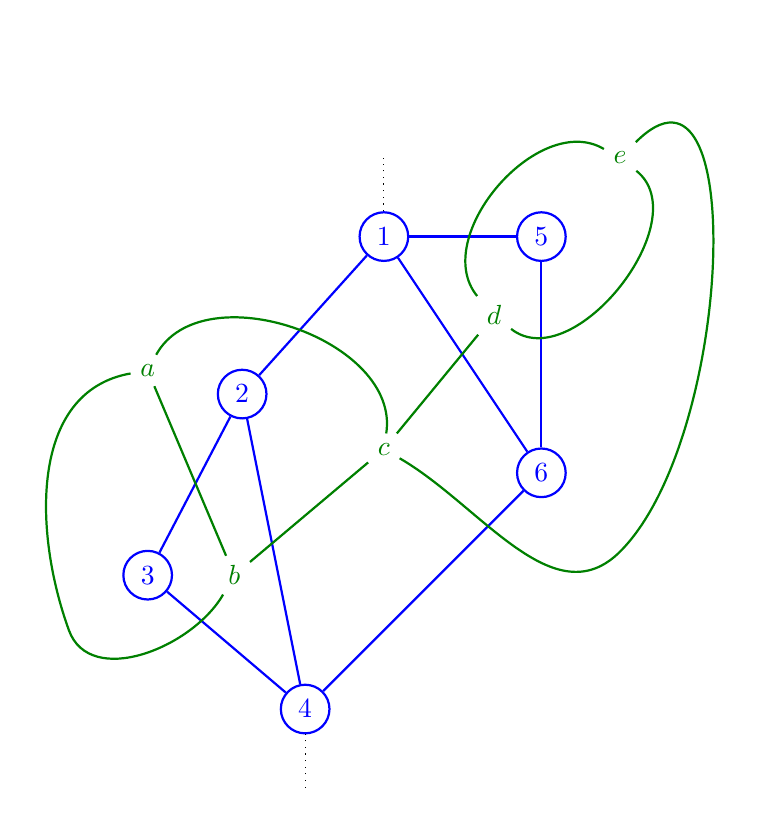
\begin{tikzpicture}[main/.style = {draw, circle, thick, color = Blue}]
			\node[main] (4) at (0,0) {4};
			\node[main] (3) at (-2,1.7) {3};
			\node[main] (6) at (3,3) {6};
			\node[main] (2) at (-0.8,4) {2};
			\node[main] (5) at (3,6) {5};
			\node[main] (1) at (1,6) {1};
			\node[color=Green] (b) at (-0.9, 1.7) {$b$};
			\node[color=Green] (a) at (-2, 4.3) {$a$};
			\node[color=Green] (c) at (1, 3.3) {$c$};
			\node[color=Green] (d) at (2.4, 5) {$d$};
			\node[color=Green] (e) at (4, 7) {$e$};
			\draw[thick, color=Blue] (4) edge (3);
			\draw[thick, color=Blue] (4) edge (2);
			\draw[thick, color=Blue] (4) edge (6);
			\draw[thick, color=Blue] (5) edge (6);
			\draw[thick, color=Blue] (6) edge (1);
			\draw[thick, color=Blue] (2) edge (1);
			\draw[thick, color=Blue] (1) edge (5);
			\draw[thick, color=Blue] (2) edge (3);
			\draw[dotted] (0, -1) -- (4);
			\draw[dotted] (1) -- (1, 7);
			\draw[thick, color=Green] (b) edge (c);
			\draw[thick, color=Green] (d) edge (c);
			\draw[thick, color=Green] (b) edge (a);
			
			\coordinate (6') at (4,2);
			\coordinate (3') at (-3, 1);
			
			\draw[thick, color=Green] (b) to[out = 240, in = -70] (3') to[out = 110, in = 190] (a);
			\draw[thick, color=Green, bend left = 80] (a) edge (c);
			\draw[thick, color=Green] (e) to[out = 45, in = 45] (6') to[out = -135, in = -30] (c);
			\draw[thick, color=Green, bend left = 80] (d) edge (e);
			\draw[thick, color=Green, bend right = 90] (d) edge (e);
		\end{tikzpicture}
	\end{subfigure}
	\begin{subfigure}{0.35\textwidth}\centering
		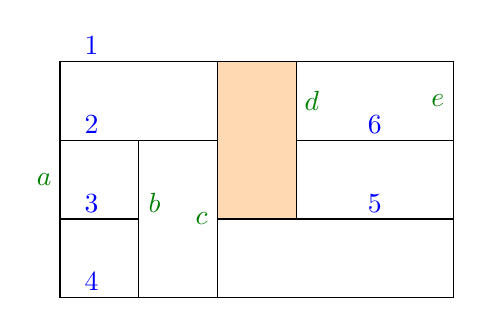
\begin{tikzpicture}
			\draw[black] (0,0) rectangle (1,1);
			\draw[black] (0,1) rectangle (1,2);
			\draw[black] (1,0) rectangle (2,2);
			\draw[black] (2,0) rectangle (5,1);
			\draw[black] (0,2) rectangle (2,3);
			\draw[black, fill=orange!30] (2,1) rectangle (3,3);
			\draw[black] (3,1) rectangle (5,2);
			\draw[black] (3,2) rectangle (5,3);
			\node[Blue] at (0.4, 3.2) {1};
			\node[Blue] at (0.4, 2.2) {2};
			\node[Blue] at (0.4, 1.2) {3};
			\node[Blue] at (0.4, 0.2) {4};
			\node[Green] at (-0.2, 1.5) {$a$};
			\node[Green] at (1.2, 1.2) {$b$};
			\node[Green] at (1.8, 1) {$c$};
			\node[Blue] at (4, 1.2) {5};
			\node[Blue] at (4, 2.2) {6};
			\node[Green] at (3.2, 2.5) {$d$};
			\node[Green] at (4.8, 2.5) {$e$};
		\end{tikzpicture}
	\end{subfigure}
	\caption{An example of a rectangle visibility representation of a planar graph. The highlighted rectangle in the representation corresponds to the primal edge 13 and dual edge $cd$.}
\end{figure}

\begin{thm}
	Every planar vertex 2-connected graph has a rectangle visibility \\ representation.
\end{thm}

\begin{proof}
	We in fact describe an algorithm how such a representation can be constructed. The bonus is that the construction runs in polynomial time.
\end{proof}

\begin{algorithm}[!ht]
	\caption{RectangleVisibilityRep}
	\begin{algorithmic}[1]
		\Require A planar graph $G$.
		\State Construct an $s - t$ numbering and a corresponding upward planar drawing as in Theorem \ref{thm-1}.
		\State Number the vertices as $1, \dots, n$ according to their $y$-coordinates (1 is the lowest vertex, $n$ is the highest one).
		\State Add a dummy arc from 1 to $n$ drawn to the right of the drawing of $G$, denote by $G'$ the resulting graph.
		\State Construct the dual graph $G^\ast$ to $G'$, and orient its edges so that each edge of $G$ is crossed by its dual edge from left to right, while the added dummy edge is crossed from right to left. Let $n^\ast$ be the number of vertices of $G^\ast$.
		\State Consider a topological sorting of the vertices of $G^\ast$ and name them $A, B, \dots$ according to this sorting.
		\State Take a grid of size $n \times n^\ast$. For a vertex $i$ of $G$, let $\alpha(\beta)$ be the face incident with $i$ with the lowest (highest, respectively) name in the topological sorting of $G^\ast$. Represent $i$ by a horizontal segment on the $i$-th line, starting at the vertical line $\alpha$ and ending on the vertical line $\beta$. For a face $\alpha$ of the drawing of $G'$ (i.e., a vertex of the dual graph $G^\ast$), let $i$ be its lowest vertex and $j$ its highest vertex (with respect to the topological sorting of $G$). Represent $\alpha$ by a segment on the vertical line $\alpha$, starting on the $i$-th horizontal line and ending on the $j$-th one.
		\State \Return this representation.
	\end{algorithmic}
\end{algorithm}

\begin{figure}[!ht]
	\begin{subfigure}{0.45\textwidth}\centering
		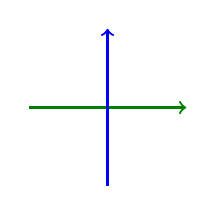
\begin{tikzpicture}
			\draw[->, color=Green, thick] (0,0) -- (2,0);
			\draw[->, color=Blue, thick] (1, -1) -- (1, 1);
		\end{tikzpicture}
	\end{subfigure}
	\begin{subfigure}{0.45\textwidth}\centering
		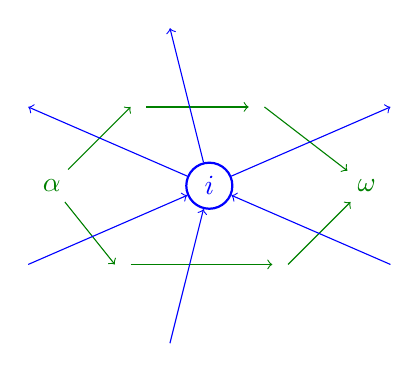
\begin{tikzpicture}
			\node[draw, circle, Blue, thick] (i) at (0,0) {$i$};
			\node[Green, thick] (a) at (-2, 0) {$\alpha$};
			\node[Green, thick] (w) at (2,0) {$\omega$};
			\draw[->, Green] (a) -- (-1, 1);
			\draw[->, Green] (-0.8,1) -- (0.5, 1);
			\draw[->, Green] (0.7, 1) -- (w);
			\draw[->, Green] (a) -- (-1.2, -1);
			\draw[->, Green] (-1, -1) -- (0.8, -1);
			\draw[->, Green] (1, -1) -- (w);
			\draw[->, Blue] (i) -- (-0.5, 2);
			\draw[->, Blue] (-0.5, -2) -- (i);
			\draw[->, Blue] (i) -- (-2.3, 1);
			\draw[->, Blue] (-2.3, -1) -- (i);
			\draw[->, Blue] (i) -- (2.3, 1);
			\draw[->, Blue] (2.3, -1) -- (i);
		\end{tikzpicture}
	\end{subfigure}
	\caption{Orientation of the dual edges (left). An example to the statement of Claim 4 (right).}
\end{figure}